%%%%%%%%%%%%%%%%%%%%%%%%%%%%%%%%%%%%%%%%%%%%%%%%%%%%%%%%%%%%%%%%%%%%%%%%
%    INSTITUTE OF PHYSICS PUBLISHING                                   %
%                                                                      %
%   `Preparing an article for publication in an Institute of Physics   %
%    Publishing journal using LaTeX'                                   %
%                                                                      %
%    LaTeX source code `ioplau2e.tex' used to generate `author         %
%    guidelines', the documentation explaining and demonstrating use   %
%    of the Institute of Physics Publishing LaTeX preprint files       %
%    `iopart.cls, iopart12.clo and iopart10.clo'.                      %
%                                                                      %
%    `ioplau2e.tex' itself uses LaTeX with `iopart.cls'                %
%                                                                      %
%%%%%%%%%%%%%%%%%%%%%%%%%%%%%%%%%%
%
%
% First we have a character check
%
% ! exclamation mark    " double quote  
% # hash                ` opening quote (grave)
% & ampersand           ' closing quote (acute)
% $ dollar              % percent       
% ( open parenthesis    ) close paren.  
% - hyphen              = equals sign
% | vertical bar        ~ tilde         
% @ at sign             _ underscore
% { open curly brace    } close curly   
% [ open square         ] close square bracket
% + plus sign           ; semi-colon    
% * asterisk            : colon
% < open angle bracket  > close angle   
% , comma               . full stop
% ? question mark       / forward slash 
% \ backslash           ^ circumflex
%
% ABCDEFGHIJKLMNOPQRSTUVWXYZ 
% abcdefghijklmnopqrstuvwxyz 
% 1234567890
%
%%%%%%%%%%%%%%%%%%%%%%%%%%%%%%%%%%%%%%%%%%%%%%%%%%%%%%%%%%%%%%%%%%%
%
%\documentclass[12pt]{iopart}
\documentclass[twocolumn,10pt]{asme2e}
%\newcommand{\gguide}{{\it Preparing graphics for IOP Publishing journals}}
%Uncomment next line if AMS fonts required
%\usepackage{iopams}  

\usepackage{epsfig} %% for loading postscript figures

	\expandafter\let\csname equation*\endcsname\relax		 %resolves conflict with amsmath package
	\expandafter\let\csname endequation*\endcsname\relax		 %resolves conflict with amsmath package
\usepackage{graphicx}
\usepackage{enumerate}
%\usepackage{subfigure}  %NOW DEPRICATED - 
\usepackage{wrapfig}
%SMS....%\usepackage{multicol}
\usepackage{booktabs}
\usepackage{multirow}
\usepackage{array}
\usepackage{amssymb,amsmath}
	\DeclareMathOperator{\sgn}{sgn}
\usepackage{epstopdf}
%\usepackage[compatibility=false]{caption}  %needed the compatibility = false command to deal with an error
\usepackage{subcaption}
%SMS....\usepackage[margin=1in]{geometry}
%SMS....\usepackage[margin=20pt,font=small,labelsep=endash]{caption}
\usepackage{url}

\confshortname{ASME SMASIS 2017}
\conffullname{the ASME 2017 Conference on Smart Materials, Adaptive Structures and Intelligent Systems}
%  \&\\
 %             Computers and Information in Engineering Conference}

%%%%% for date in a single month, use
\confdate{18-20}
\confmonth{September}
%%%%% for date across two months, use
%\confdate{August 30-September 2}
\confyear{2017}
\confcity{Snowbird, UT}
\confcountry{USA}

%%% Replace DETC2010/MECH-12345 with the number supplied to you 
%%% by ASME for your paper.
\papernum{SMASIS2017-3803}


\title{A novel biomimetic torsional actuator design using \\ twisted polymer actuators}

%%% first author
\author{Michael W. Shafer
    \affiliation{ 
	Assistant Professor\\
	Dept. of Mechanical Engineering\\
	Northern Arizona University\\
	Flagstaff, Arizona 86001\\
    Email: Michael.Shafer@nau.edu
    }
}

\author{Heidi P. Feigenbaum
    \affiliation{ 
	Associate Professor\\
	Dept. of Mechanical Engineering\\
	Northern Arizona University\\
	Flagstaff, Arizona 86001\\
    Email: Heidi.Feigenbaum@nau.edu
    }
}

\author{Diego Ricardo Higueras Ruiz 
    \affiliation{ 
	M.S. Candidate \\
	Dept. of Mechanical Engineering\\
	Northern Arizona University\\
	Flagstaff, Arizona 86001\\
      Email: dr779@nau.edu
    }
}


\begin{document}

\maketitle    

\begin{abstract}

Artificial muscle systems have the potential to impact many technologies ranging from advanced prosthesis to miniature robotics. Recently, it has been shown that twisting drawn polymer monofilaments, such as nylon fishing line or sewing thread, can result in a biomimetic thermally activated torsional actuator. The actuation phenomenon in these twisted polymer actuators (TPAs) is thought to be a result of an untwisting that occurs about the fiber's axis due to an asymmetric thermal expansion. Before being twisted, the precursor fibers are comprised of polymer chains that are aligned axially. During fabrication of TPAs, the polymer chains reorient as the precursor fiber is twisted about the central axis of the monofilament.  At the end of the fabrication process, the TPA is annealed in order to relieve internal stresses and to keep the fiber in the twisted configuration. Upon heating the (untwisted) precursor fiber, it expands radially and contracts axially. After being twist, these radial and axial expansion relationships remain relatively unchanged, but the polymer chain direction is no longer axially aligned. Thus, upon heating the twisted fibers of the TPA, the fibers untwist and torsional actuation occurs.  This result is similar to the effect one would expect when inflating a cylindrical balloon that has been helically wrapped with an inextensible string. As the balloon inflates, the string (i.e. the polymer chain) cannot stretch, so it must untwist on the balloon as the helical circumference it is wrapped around increases. 

Compared to other torsional actuators TPAs are low cost, lightweight, and can actuate reasonably high torques per unit volume.  However, because TPAs are thermally activated, they may not be suitable for all applications. 

In this work, we present a novel TPA design for use as a torsional actuator for miniature actuation and artificial muscle applications. Our design bundles twisted monofilaments to increase the torque. Both fabrication and testing methods of the new design are presented.  Results for temperature versus torsional displacement under various loads give insights as to how these actuators may be used and the reversibility of the actuation process.  

%with heating wire to supply the temperature change and induce actuation. The conceptual design of this novel torsional actuator is presented here, along with the unloaded free rotation response of various configurations. Experimental characterization of the design includes direct temperature measurements of the TPA using an attached thermocouple, and  torsional displacement measured using video recordings of the actuation.  Results of these tests are presented and comparisons are made between the various configurations. Based on these results, we suggest further improvements that could be made to the design of these torsional actuators.  
\end{abstract}

% Uncomment for PACS numbers
%\pacs{00.00, 20.00, 42.10}
%
% Uncomment for keywords
%\vspace{2pc}
%\noindent{\it Keywords}: XXXXXX, YYYYYYYY, ZZZZZZZZZ
%
% Uncomment for Submitted to journal title message
%\submitto{\JPA}
%
% Uncomment if a separate title page is required
%\maketitle
% 
% For two-column output uncomment the next line and choose [10pt] rather than [12pt] in the \documentclass declaration
%\ioptwocol
%


\section{Introduction}
%The apparent simplicity of drawn polymer monofilaments has until recently hidden their capacity for work as an actuator. 
It was recently shown that drawn polymers monofilament such as nylon fishing line have the ability to act as linear actuators when twisted and configured helically if exposed to temperature changes \cite{haines_artificial}. The same monofilaments can be torsional actuators if twisted but not coiled heliccally \cite{haines_artificial}.  In the pursuit of an thermo-mechanical actuation model for these twisted polymer systems, our group has looked toward understanding how twisted polymer monofilaments would react torsionally when exposed to temperature changes \cite{shafer_first}. As part of this modeling effort, concepts in torsional actuation configurations were conceived. This work presents conceptual designs and actuation performance for a torsional actuator based on two configurations of a twisted polymer actuator (TPA). 

Twisted polymer actuators, when configured to act as a linear actuator, are often classified as a type of artificial muscle. A wide variety of artificial muscle technologies exist for linear actuation. While less work has focused on how smart materials can be configured for torsional actuation, there are still a number of materials in use. Some of these technologies use a linear actuation phenomenon in a helical configuration to induce a twisting. Nitinol shape memory alloys (SMA), typically used for linear actuation, have been used in a tube configuration to create a torsional actuator [3***]. Many other torsional actuation technologies rely on  radial changes of materials in helical configurations. Electroactive polymers, pneumatic and hydraulic artificial muscles, and carbon nanotubes, have all been used in a helical configuration to create torsional actuation through radial changes [1, 2, 5, 6]. While the method of radial changes varies between materials, the mechanism of actuation remains the same and relies on increasing the path length for helically wrapped fibers. Each of these technologies has impressive performance in at least one metric, but none are as simple and inexpensive as torsional twisted polymer actuators (TPAs).

In discussing these polymer actuators, it is important to make clear the differences in terminology regarding `twist' and `coil'. A precursor fiber is considered to be a straight drawn polymer fiber, such as monofilament fishing line, while a twisted fiber is one in which a precursor fiber is twisted about its central axis but remains straight. Although a twisted precursor fiber will remain straight, after twisting its polymer chains will be helically oriented about the precursor fiber's axis with a pitch angle that depends in radial position. Figure \ref{fig:helix} highlights how twisting reorients the polymer chains into a helical configuration with a radially dependent pitch. Typically, after twisting the material is annealed so that internal stresses are relieved and the material remains twisted when unloaded. Coiling refers to a fiber, twisted or untwisted, that is annealed in a helical configuration. This helical configuration can be developed by increasing the amount of twist in a precursor fiber to a point at which the fiber torsionally buckles and coils over on itself, or helically wrapping on a mandrel. With these definitions for `twisting' and `coiling,' we use the terms `straight-twisted polymer actuators' (STPA) to refer to the torsional actuators that are not coiled, and `twisted-coiled polymer actuators' (TCPA) to refer the linear actuators in the helical configuration. 

Individual straight twisted polymer actuators can be used to generate low torque torsional actuations similar to the way in which CNT yarns have been used in the past [1***], but at significantly lower cost. In this work, we present isotonic torsional actuation performance for such a monofilament STPA configuration. We also consider here the configuration of STPAs wrapped into a parallel configuration such that multiple STPAs work together to generate a torque. This configuration can be seen in Figure [ADD REF TO FIGURE HERE]. Such a configuration is fabricated using standard rope making manufacturing processes, and as such, allows for a wide variety of potential configurations of parallel STPA elements, structural elements, and heating elements. The isotonic concentric and eccentric actuation performance of these parallel STPA configurations are shown. As part of this study, we present the fabrication techniques for monofilament STPAs and parallel STPAs. We also show how a core can be added to the the parallel configuration in order to for direct heating of the actuator from within the actuator. The stroke-temperature relationship is investigated for both monofilament and parallel actuator designs for three different preload torques. 

% [1] Torsional Actuator Powered by Environmental Energy Harvesting from Diurnal Temperature Variation Dongseok Suh, Thuy Kieu Truong, Daniel G. Suh,  and Seong Chu Lim. Department of Energy Science, Sungkyunkwan University, Suwon 16419, Korea
%The Alan G. MacDiarmid NanoTech Institute, University of Texas at Dallas, Richardson, Texas 75083, United States
%
%[2] Hybrid carbon nanotube yarn artificial muscle inspired by spider dragline silk. Kyoung-Yong Chun, Shi Hyeong Kim, Min Kyoon Shin, Cheong Hoon Kwon, Jihwang Park, Youn Tae Kim, Geoffrey M. Spinks, Marcio D. Lima, Carter S. Haines, Ray H. Baughman & Seon Jeong Kim.
%
%[3] Shape Memory Alloy TiNi Actuators for Twist Control of Smart Wing Designs. A. Peter Jardine, Jayanth N. Kudva, Christopher Martin and Kari Appa, Northrop-Grumman Corp.
%[4] First steps in modeling thermal Actuation of Twisted Polymer Actuators using virgin material properties. Michael W. Shafer, Heidi P. Feigenbaum, Daniel Pugh & Matthew Fisher.
%
%[5] Fiber-Directed Conjugated-Polymer Torsional Actuator: Nonlinear Elasticity Modeling and Experimental Validation Yang Fang, Member, IEEE, Thomas J. Pence, and Xiaobo Tan, Member, IEEE
%
%[6] Pneumatic Torsional Actuators for Inflatable Robots. Siddharth Sanan Peter S. Lynn Saul T. Griffith. Carnegie Mellon University
%
%[7] Analytical study on torsion of shape-memory-polymer prismatic bars with rectangular cross-sections. M. Baghani. School of Mechanical Engineering, College of Engineering, University of Tehran, P.O. Box 11155-4563, Tehran, Iran
% 
 
%	
%	A variety of technologies and materials have been proposed as artificial muscles. Shape-memory alloys (SMA) are a type of ``smart-material'' that can return to a preset shape after some mechanical deformation and thereby act as an actuator. Spun carbon nanotube (CNT) yarns have also been employed as synthetic muscles \cite{lima_electrically, foroughi_torsional} . The expense of SMAs and CNT yarns impede wide scale deployments of the technologies. Conversely, it was recently discovered that extremely inexpensive drawn polymer monofilaments, such as nylon and polyethylene that are used in fishing line, have anisotropic thermal expansion characteristics and can actuate similarly to CNT yarns. By twisting and coiling the fishing line, extremely powerful, lightweight, and inexpensive thermally-activated actuators can be made whose specific load capacity is higher than human muscle \cite{haines_artificial}. %
%	
%	In discussing these actuators, it is important to understand the differences in terminology regarding twist and coiling. A precursor fiber is considered to be a straight drawn polymer fiber, while a twisted fiber is one in which a precursor fiber is twisted about its central axis but remains straight. Although a twisted fiber will remain straight, after twisting its polymer chains will then be helically oriented about the fiber axis with a pitch angle that depends in radial position (see Fig. \ref{fig:helix}). Typically, after twisting the material is annealed so that internal stresses are relieved and the material remains twisted when unloaded. Coiling refers to a fiber, twisted or untwisted, that is annealed in a helical configuration. This helical configuration can be developed by increasing the amount of twist in a precursor fiber to a point at which the fiber torsionally buckles and coils over on itself. Alternatively, a twisted or untwisted fiber can be wrapped around a mandrel prior to annealing. %The thermal annealing process is typically employed to relieve internal stresses so that a twisted or coiled configuration remains when fabrication torques and forces are removed. 
%	Depending on the final configuration of the polymer fiber, a variety of combinations are possible, but the most typical would be twisted-coiled polymer actuators (TCPAs) which provide linear actuation and twisted polymer actuators (TPAs) which provide torsional actuation. 

%\begin{figure}
%    \centering
%   % \begin{subfigure}[b]{0.3\textwidth}
%        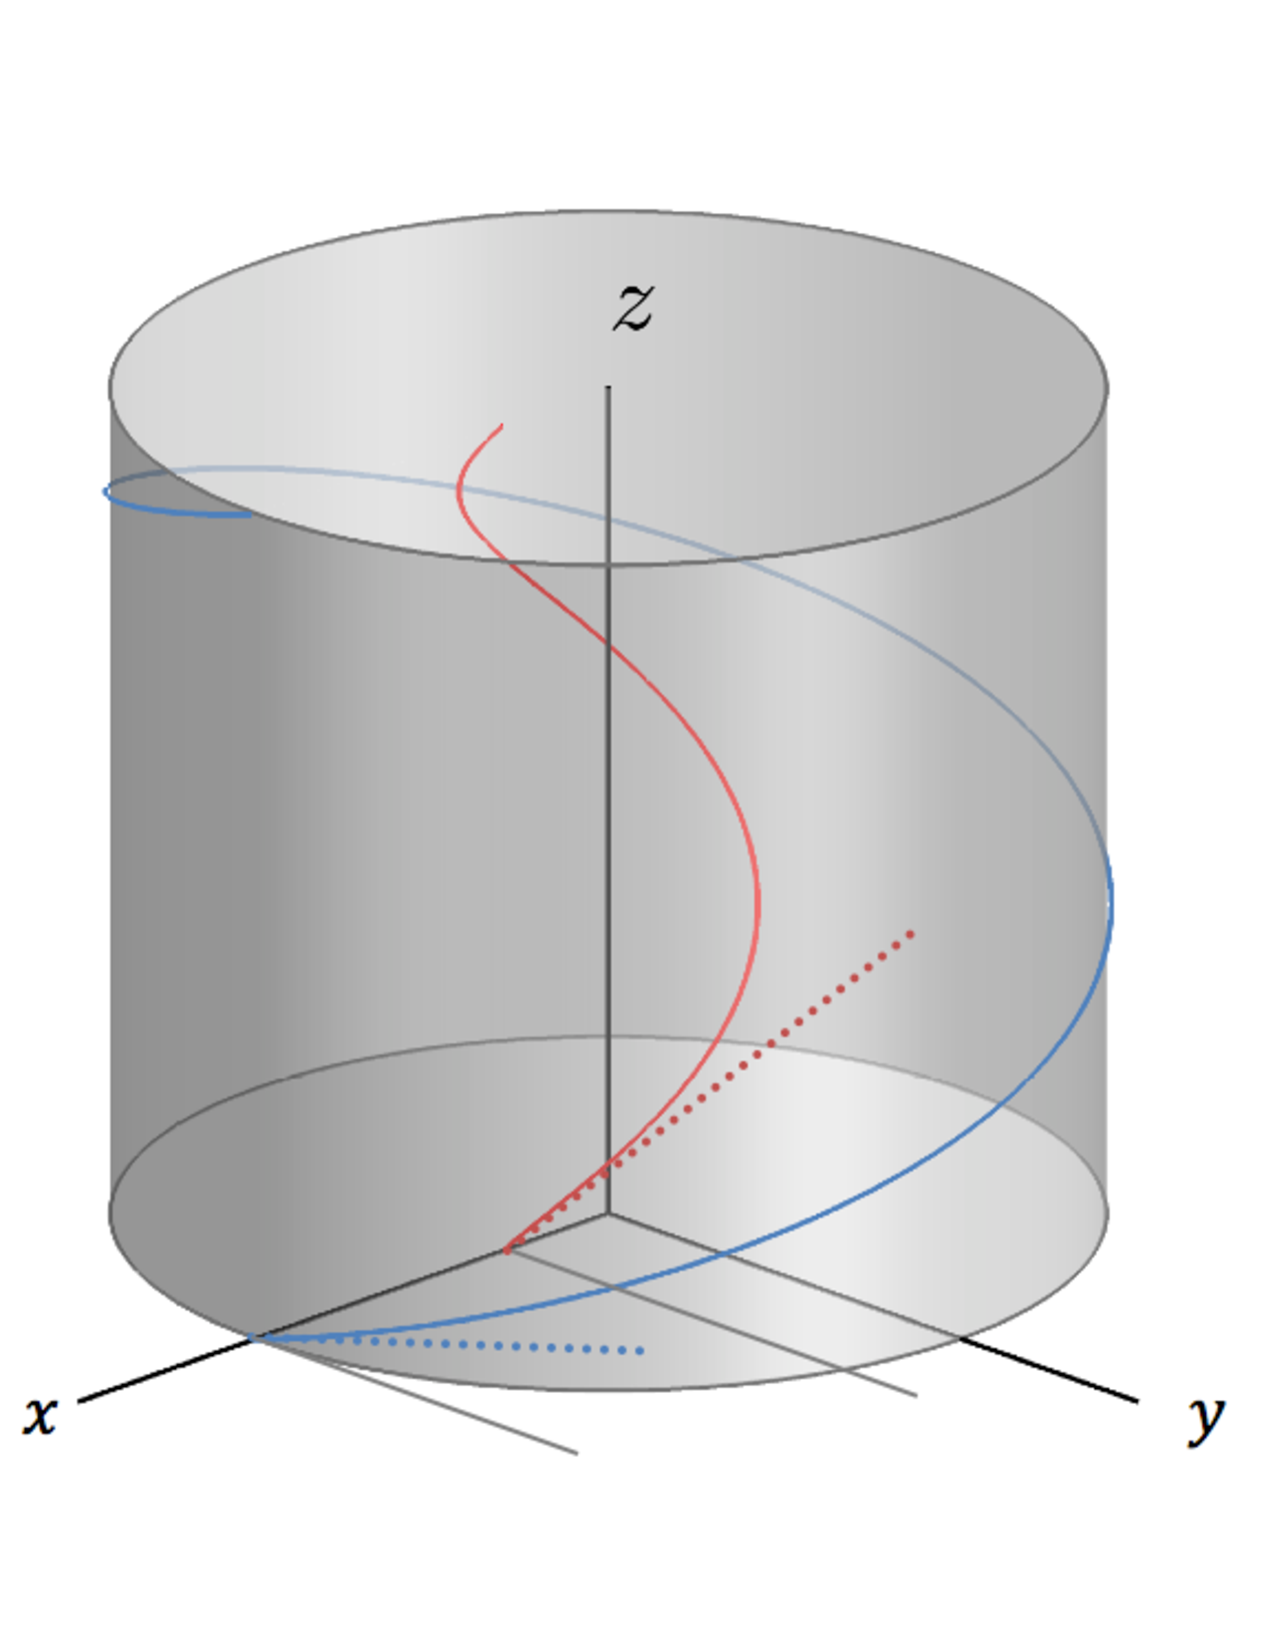
\includegraphics[width=6cm, clip = true, trim = {0in 0in  0in 0in}]{../Images/helix.pdf}
%        \caption{Twisted monofilament with lines representing polymer chain configurations after inserted twist.}
%        \label{fig:helix}
%				%%%% I like this figure but I want to adjust it - it shouldn't be r theta, it should be x & y on the horizontal axis and maybe label alpha in the picture too.  
%				
%				
%    %\end{subfigure}
%  %  \quad %add desired spacing between images, e. g. ~, \quad, \qquad, \hfill etc. 
%      %(or a blank line to force the subfigure onto a new line)
%   % \begin{subfigure}[b]{0.5\textwidth}
%    %    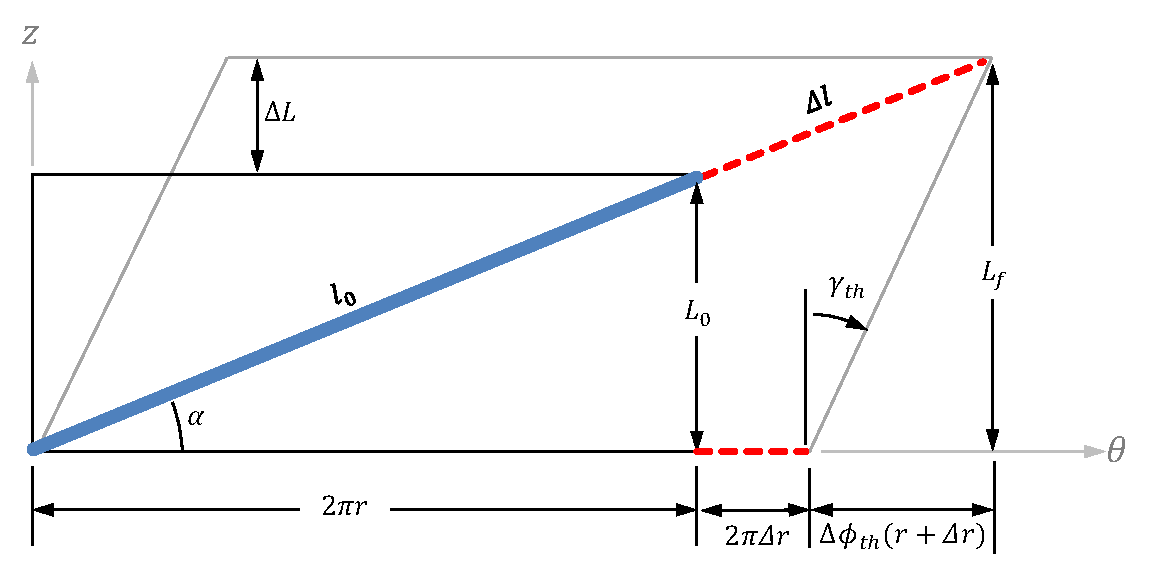
\includegraphics[width=9cm,]{../Images/1D_thermal_kinematic_v2.pdf}
%     %   \caption{}
%     %   \label{fig:1D_thermal}
%    %\end{subfigure}
%    %\caption{(\subref{fig:helix}) A section of precursor fiber after inserting twists. Polymer chains highlighted in blue showing variable angle as a function of radius. (\subref{fig:1D_thermal}) Polymer chain before and after heating with shear modulus assumed to be negligible. Dark blue line is original length of single wrap of polymer chain at some radial position. Untwist angle $\phi_{th}$ shown as negative because positive angles are taken as twists about the $z$-axis of the fiber}
%  %  \label{fig:1D_conceptual}
%\end{figure} 

%\begin{figure}
%    \centering
%   % \begin{subfigure}[b]{0.3\textwidth}
%        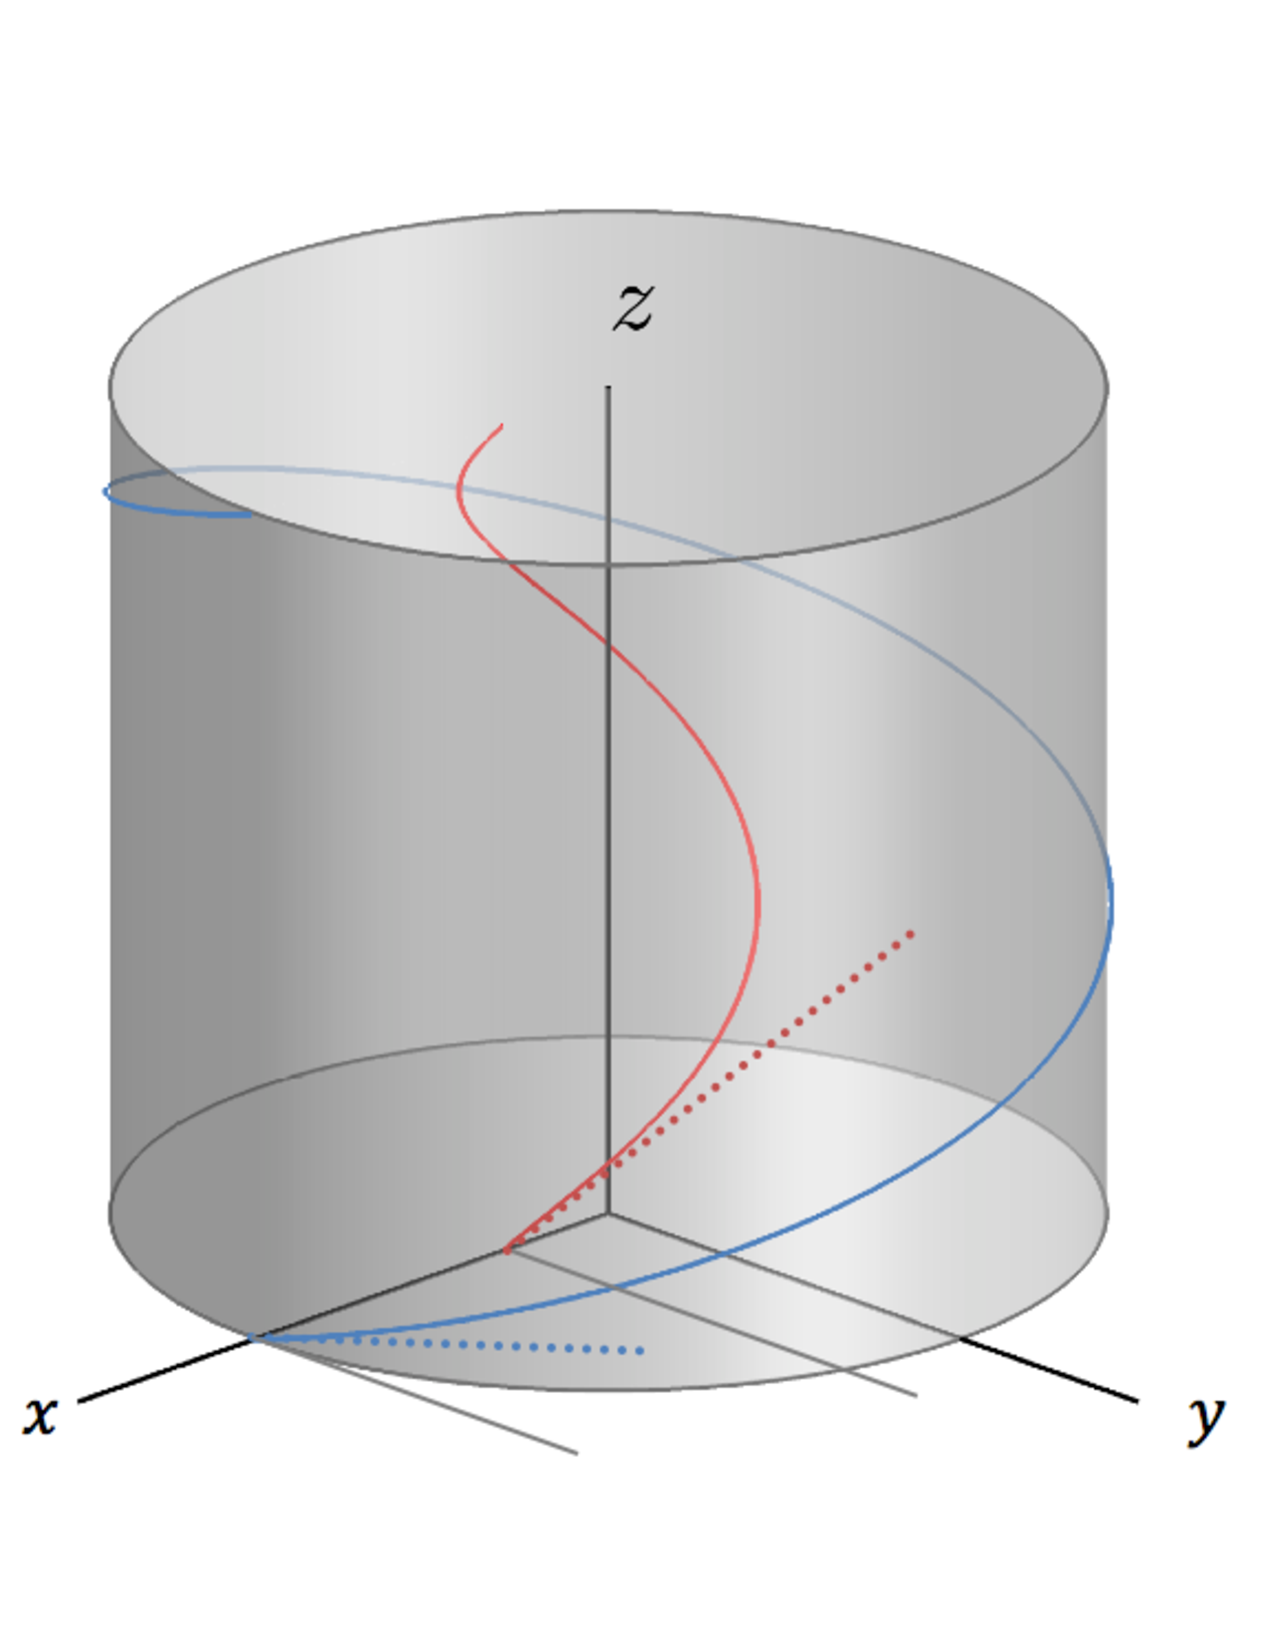
\includegraphics[width=6cm, clip = true, trim = {0in 0in  0in 0in}]{../Images/helix.pdf}
%        \caption{Twisted monofilament with lines representing polymer chain configurations after inserted twist.}
%        \label{fig:helix}
%\end{figure} 
%
%

%\begin{figure}
%    \centering
%     \begin{subfigure}[b]{0.5\textwidth}
%        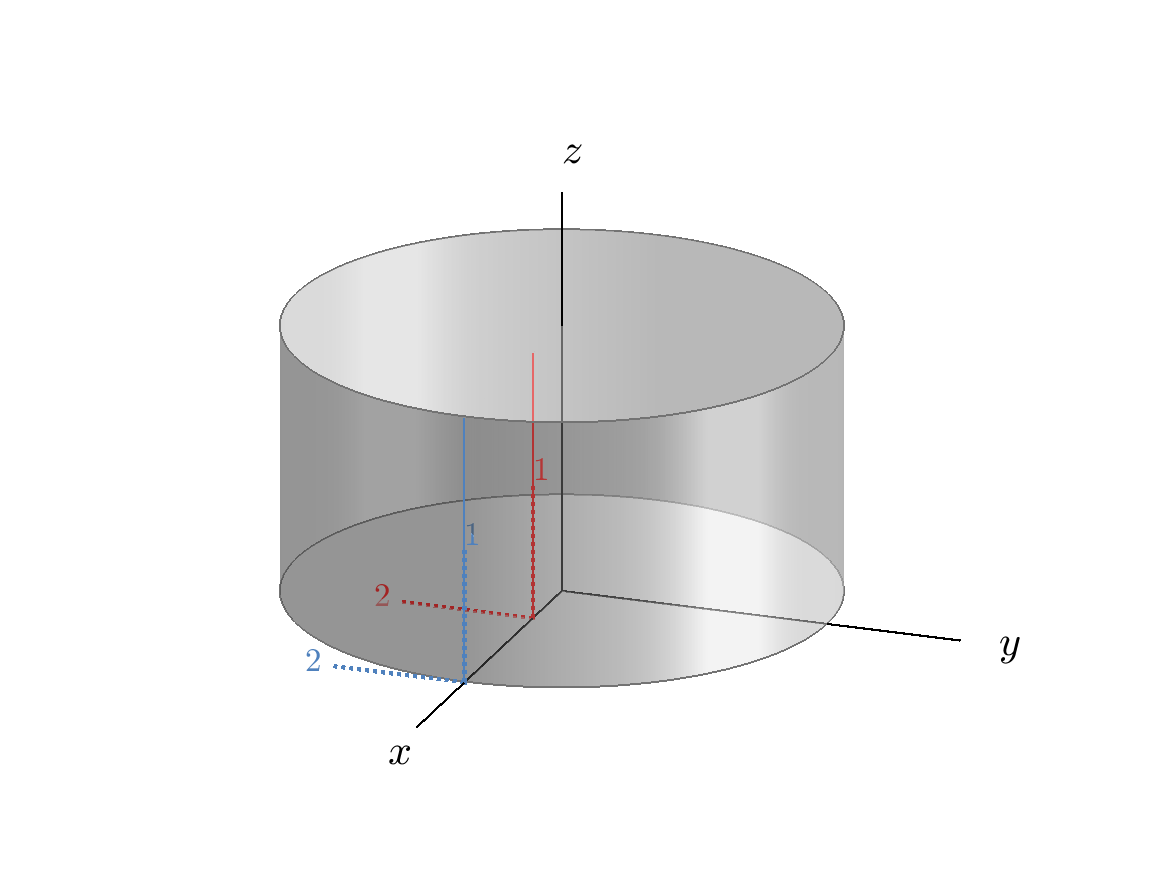
\includegraphics[width=9cm, clip = true, trim = {1in 1in  1in 1in}]{../Images/helix_2_initial.pdf}
%        \caption{Initial configuration }
%        \label{fig:helix_init}
%        \end{subfigure}
%     \begin{subfigure}[b]{0.5\textwidth}
%        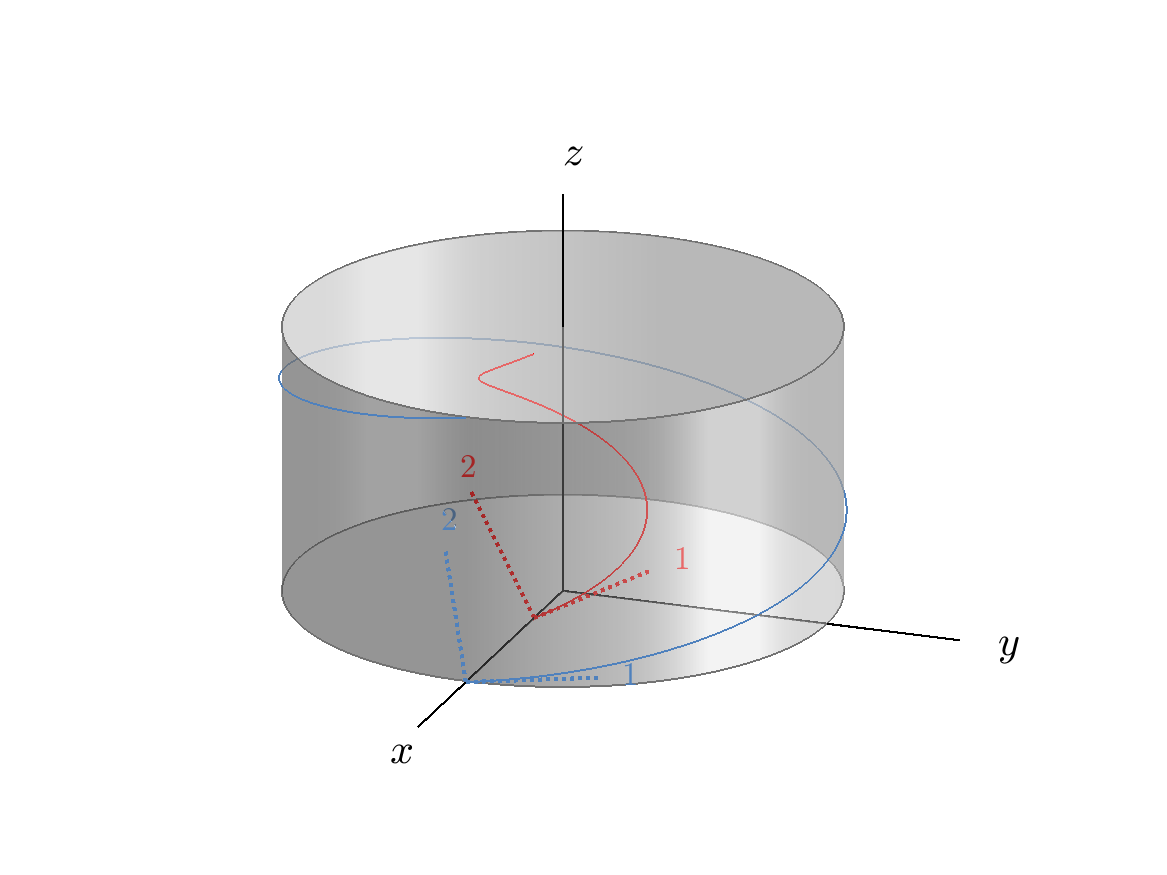
\includegraphics[width=9cm, clip = true, trim = {1in 1in  1in 1in}]{../Images/helix_2.pdf}
%        \caption{Twisted and annealed configuration}
%        \label{fig:helix_final}
%        \end{subfigure}
%        \caption{Conceptual diagram showing (\subref{fig:helix_init}) untwisted and (\subref{fig:helix_final}) twisted monofilament with lines representing polymer chain configurations. Notices that angle of polymer chain with respect to the $x-y$ place depends on radial position after twisting, but not before.}
%        \label{fig:helix}
%\end{figure}
%
\begin{figure}
    \centering
     \begin{subfigure}[b]{0.5\textwidth}
        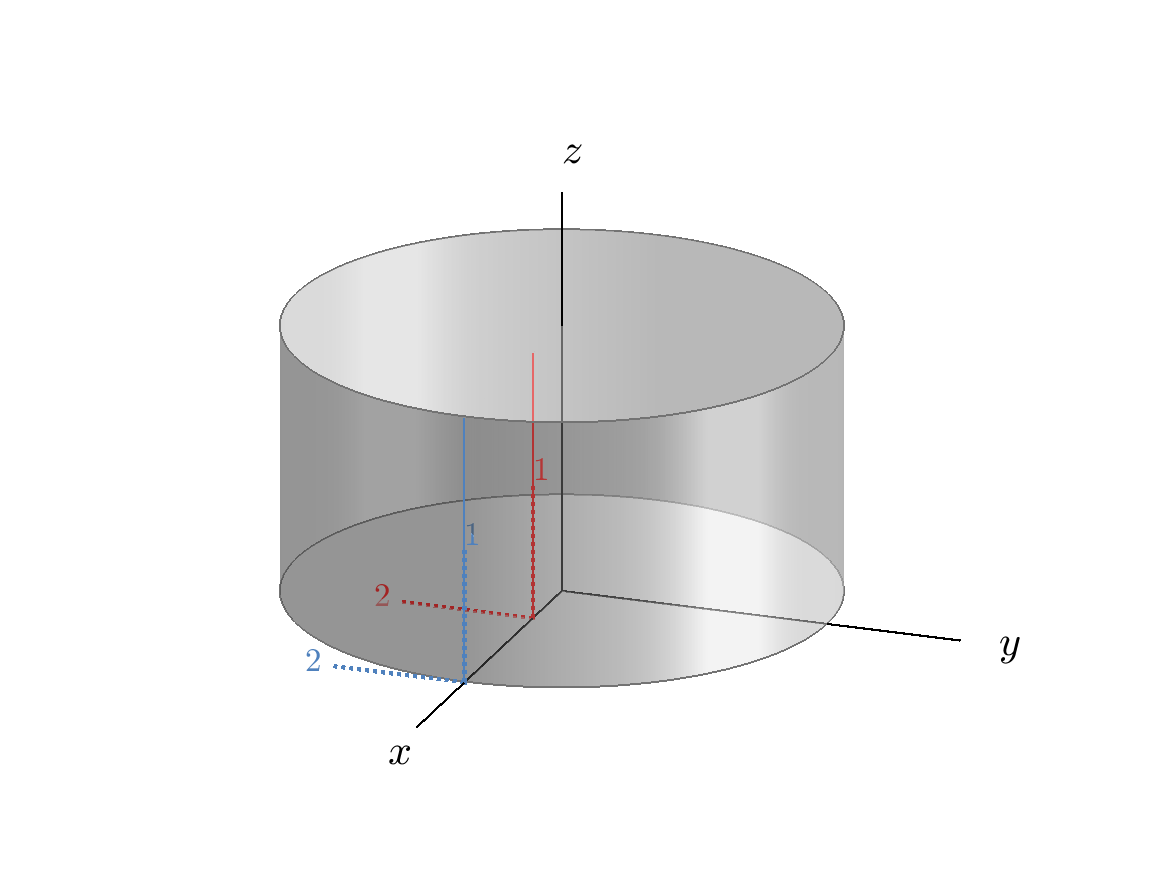
\includegraphics[width=7cm, clip = true, trim = {0.8in 0.5in  0.8in 0.8in}]{../Images/helix_2_initial.pdf}
        \caption{Initial configuration }
        \label{fig:helix_init}
        \end{subfigure}
     \begin{subfigure}[b]{0.5\textwidth}
        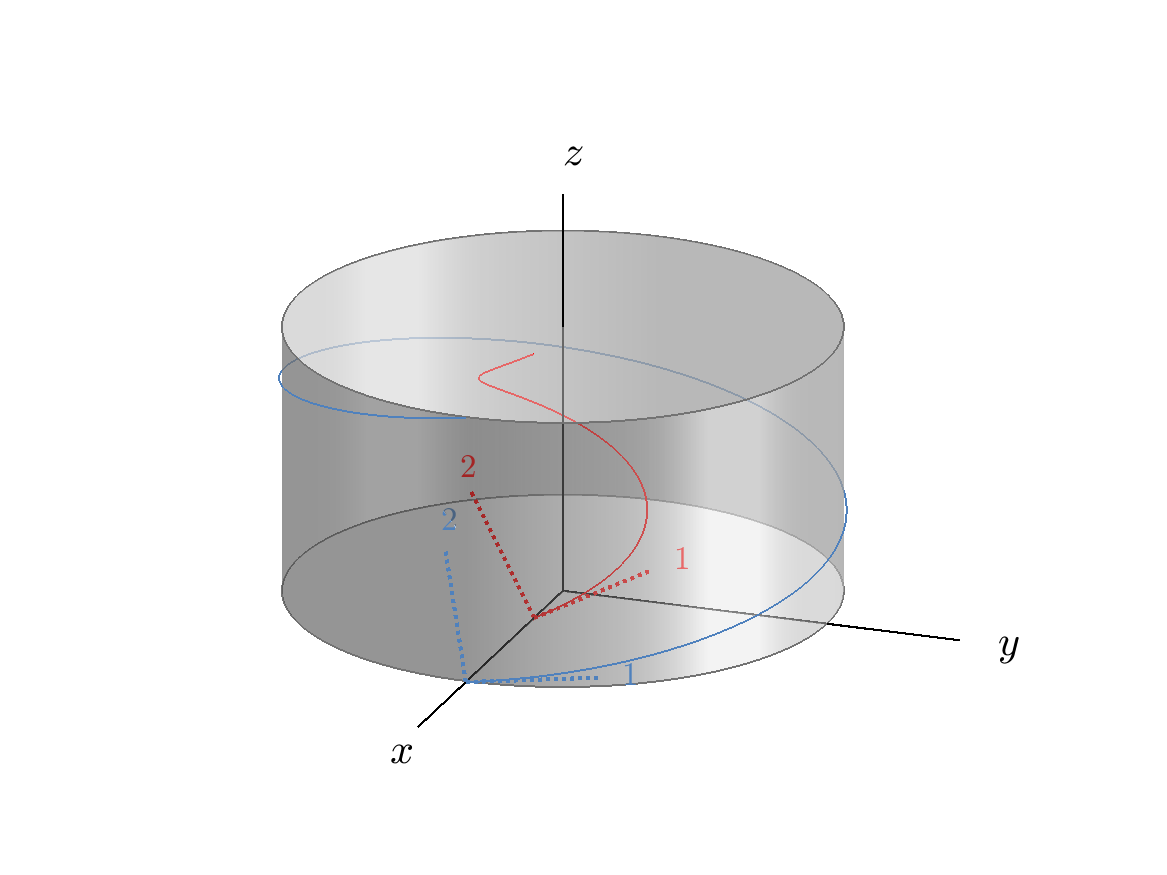
\includegraphics[width=7cm, clip = true, trim = {0.8in 0.5in  0.8in 0.8in}]{../Images/helix_2.pdf}
        \caption{Twisted and annealed configuration}
        \label{fig:helix_final}
        \end{subfigure}
        \caption{Conceptual diagram showing (\subref{fig:helix_init}) untwisted and (\subref{fig:helix_final}) twisted monofilament with lines representing polymer chain configurations. Notices that angle of polymer chain (1-direction) with respect to the $x-y$ plane ($\alpha$) depends on radial position after twisting.}
        \label{fig:helix}
\end{figure}


% \begin{figure*}
%    \centering
%   % \begin{subfigure}[b]{0.3\textwidth}
%%        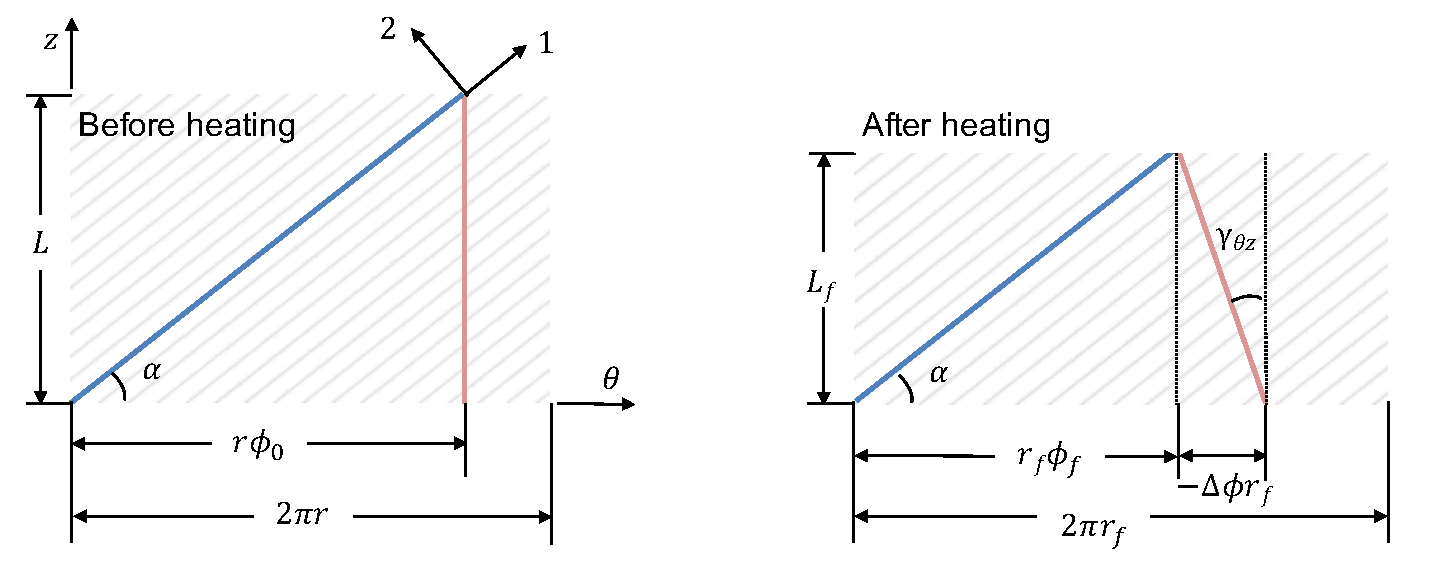
\includegraphics[width=15cm ]{../Images/unwrapped_2_both.pdf}
%        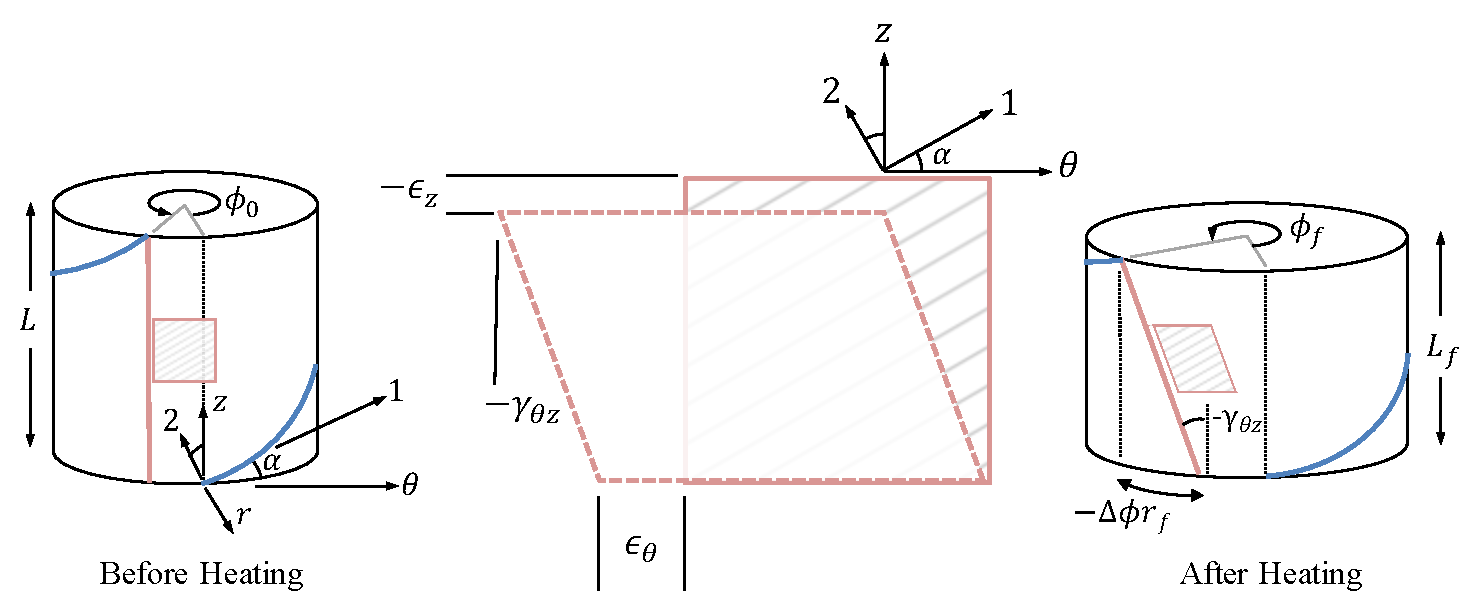
\includegraphics[width=14cm , clip = true, trim = {0in 0in  0in 0.1in}]{../Images/elemental_diagram_2}
%        \caption{Sections of TPA before and after heating with elemental 2D section shown on both, as well as enlarged between the two. The elemental section shows shear, axial, and tangential strains resulting from thermal loading of a twisted polymer. Radial ($r$), tangential ($\theta$) and axial ($z$) coordinates, as well as the polymer chain coordinates (1 \& 2 directions) are shown. Notice that 1 and 2 directions are rotated from $\theta$ and $z$ directions by angle $\alpha$.  This rotation is due to the initial twist angle shown as $\phi_0$, which is maintained due to annealing.  The initial angle $\phi_0$ is changed to $\phi_f$ after heating as a result of a thermally induced twisting by angle $-\Delta\phi$.}
%        \label{fig:unwrapped}
%\end{figure*}
%
%
%To date, research on TPAs and TCPAs has focused on experimentally exploring the actuation phenomenon and characterizing actuator performance \cite{haines_artificial, mirvakili_simple, cherubini_experimental, moretti_experimental}. Due in part to the novelty of these devices, the complex geometry of the coiling, and the experimental challenges in model validation, there is limited work on the analytic modeling of these synthetic actuators.  Because of their simpler geometry, the modeling work to date has focused on TPAs rather than TCPAs. 
%Aziz et al. \cite{aziz_controlled} used the thermal expansion properties of twisted fibers along with classical torsion theory to model TPAs and got good agreement with experimental results for both torsional stroke, i.e. untwist, and blocked torque, i.e. torque that develops when the heated fibers are securely clamped.  However, using thermal expansion of the twisted fibers for design purposes can be limiting because it requires experimental tests whenever a new initial twist is inserted.  Additionally, their work assumed no length changes in the twisted fibers. 
%
%\begin{figure}
%    \centering
%   % \begin{subfigure}[b]{0.3\textwidth}
%        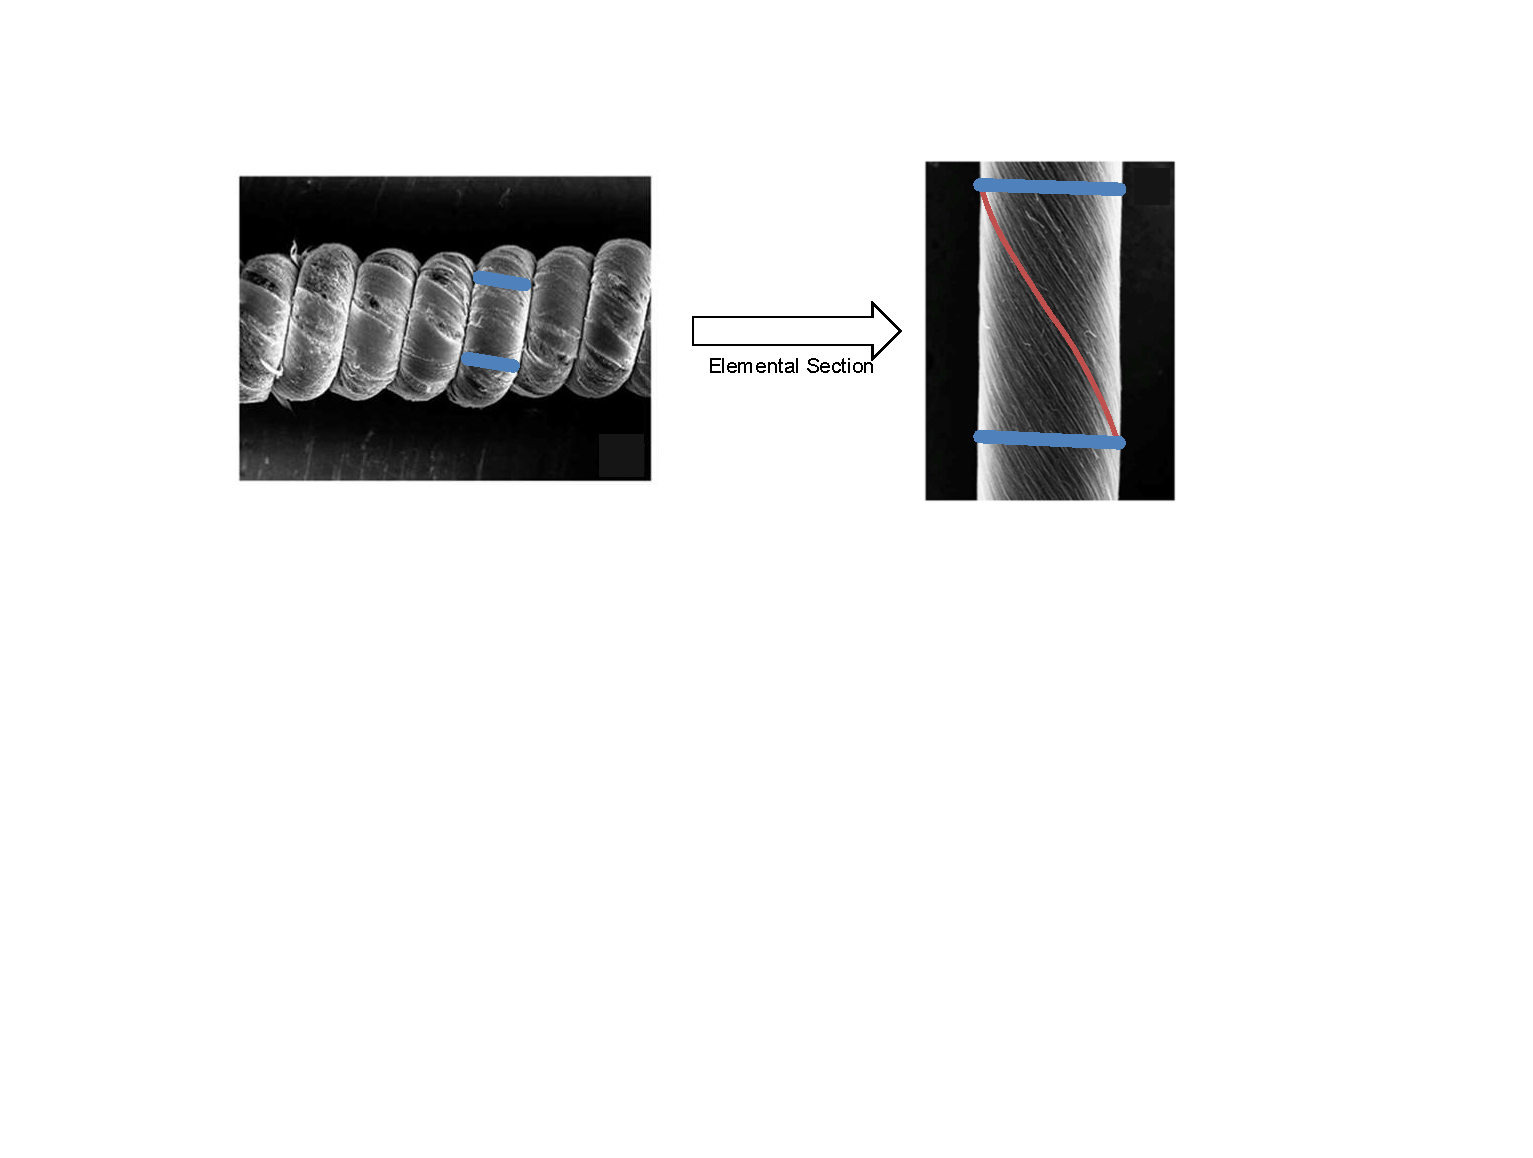
\includegraphics[width=9cm, clip = true, trim = {1in 3.5in  1in 0.5in}]{../Images/coiled.eps}
%        \caption{Twisted coiled polymer actuator (TCPA) on the left and twisted polymer actuator (TPA) on the right which can be considered an elemental section of the TCPA. Adapted from [Haines et al. 2014].}
%        \label{fig:coiled}
%\end{figure}
%


\section{Fabrication of torsional twisted polymer actuators}
Straight fiber
Parallel configuration


\begin{figure}
    \centering
     \begin{subfigure}[b]{0.15\textwidth}
        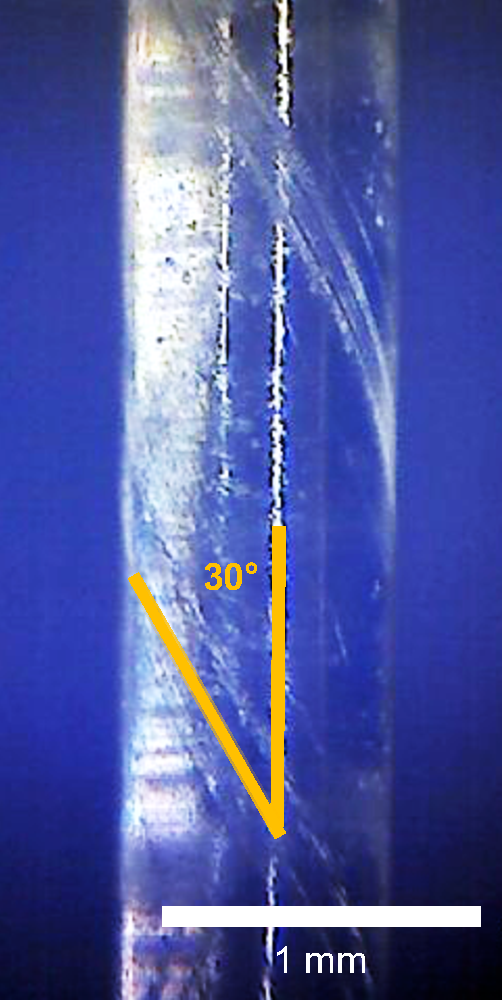
\includegraphics[width=3.5cm]{../Images/micro_mono.pdf}
        \caption{}
        \label{fig:miro_mono}
        \end{subfigure}
        \quad \quad  \quad \quad
     \begin{subfigure}[b]{0.15\textwidth}
        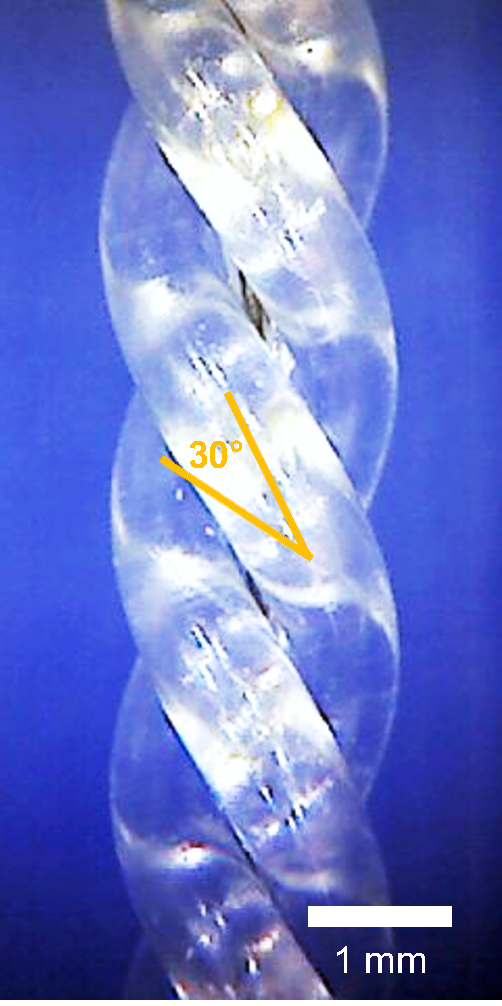
\includegraphics[width=3.5cm]{../Images/micro_para.pdf}
        \caption{}
        \label{fig:micro_para}
        \end{subfigure}
        \caption{Microscope images showing (a) an monofilament STPA with pitch angle of $30^\circ$ and (b) a parallel STPA actuator with the same pitch angle as the monofilament configuration. Also visible in (b) is how a NiCr heater wire element can be spliced within the parallel STPA configuration.  }
        \label{fig:micro}
\end{figure}


\begin{figure}
    \centering
        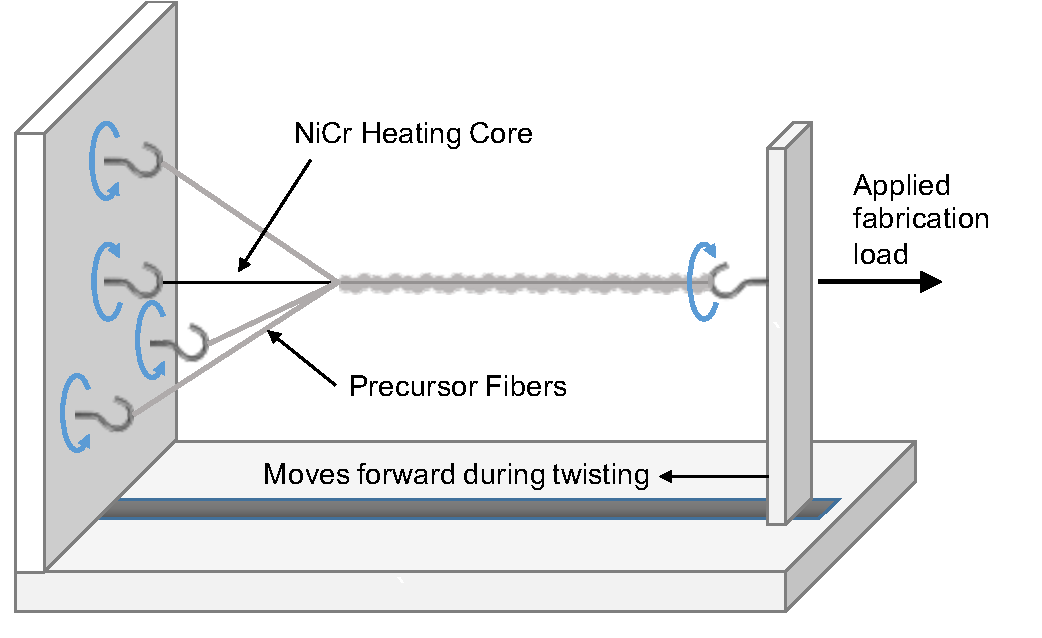
\includegraphics[width=8cm]{../Images/coiling_rig.pdf}
        \caption{Fabrication rig for torsional TPA based on twisted rope fabrication process. During the twisting process the precursor fibers are twisted in a direction opposite to that of the hook on the right. If a central heating or structural core is use, the center hook on the left is turned at the same rate as that on the right to maintain zero twist in the core. }
        \label{fig:coiled}
\end{figure}

\section{Methods for isotonic torsional stroke testing}
In order to characterize these torsional actuators, an experimental setup was designed and built which maintained a constant torque on the actuators during heating. A preload torque is known to be required to bring these actuators back to their initial angle state after cooling. The experimental setup included a 3D printed frame, ball bearing, torque spool, clamp, and weight. This setup can be see in figure \ref{fig:setup}. In this figure, the actuator sample can be seen to be clamped on the right of the frame. The left side of the sample is glued into the torque spool, a hollow pulley that interfaces with a bearing pair. A pair of ball bearings are used to react both the moment and radial loads passed into the torque spool from the weight. This weight hangs from the 6 mm diameter torque by a fine steel wire. 

The position of the weight is measured using a Polytec OVF-5000/OVF-534 vibrometer controller and sensor unit, along with DD-900 Digital Displacement Decoder unit. The voltage output of this system is linearly related to a change of position of the object on which it focuses. This voltage is recorded by a National Instruments PXI-XXXX multifunction data acquisition card, which simultaneously samples temperature measurement from the K-type thermocouple embedded within the test sample as shown in figure \ref{fig:setup}. Ambient room temperature is noted from the sample temperature prior to the application of a thermal load. Temperature and displacement measurements are recorded at 100 Hz. 

Each test is initiate by clamping an actuator sample in a frame and applying a preload torque by attaching a weight to the cable on the torque spool. The laser vibrometer zero position is then reset, and the data acquisition system is started. A hot air source is then placed adjacent to the sample to heat the actuator. When the temperature of the actuator reaches between 90-100$^\circ$C the heat source is removed, as temperatures above 120$^\circ$C are known to anneal the nylon precursor fibers. The actuator is then allowed to cool under free convection until the internal temperature returns to the pre-heating condition. 


\begin{figure}
    \centering
        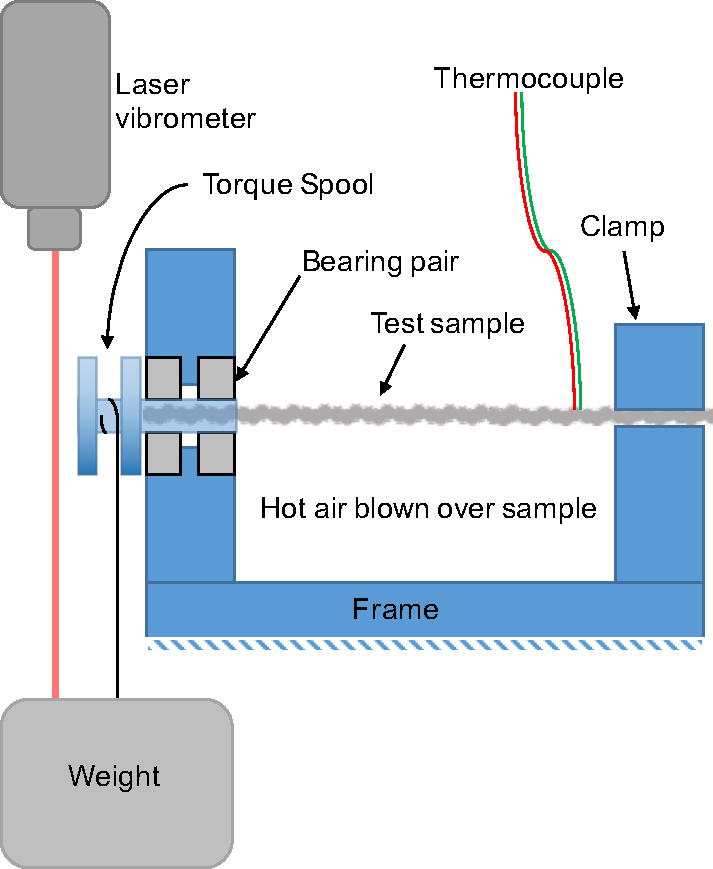
\includegraphics[width=6cm]{../Images/experimental_setup.pdf}
        \caption{Isotonic experimental testing rig for measuring actuation stroke under thermal loading.}
        \label{fig:setup}
\end{figure}

\section{Experimental Results}
For each torque preload, five heating cycles were conducted while measuring actuation angle. The time histories of the heating and cooling of two torque preloads are shown in figure \ref{fig:time_hist_m} for a monofilament STPA and figure \ref{fig:time_hist_p} for the parallel configuration. Because the parallel configuration used three twisted monofilaments, three times the preload torque was applied to the parallel configuration tests allow for direct comparison between the monofilament and parallel configuration. A constant torque of 0.883 N-mm and 2.94 N-mm were applied for the monofilament heating cycles while 2.94 N-mm and 8.83 N-mm were applied for the parallel configuration heating cycles. In these figures, the response of these actuators to changes in temperature can be seen. The long cooling period, on the order of 200 s, is due to the reliance on free convective cooling in the ambient environment.

Initial trials indicated that for low preloads in both the monofilament and parallel actuator testing, there is an initially large actuation angle which is not fully recoverable. This evident in the first graph of figure \ref{fig:time_hist_m}. In this figure, the an initial displacement angle of approximately $27^\circ$ is achieved, but only slightly more than $5^\circ$ are recoverable, and a permanent deformation is present after cooling. This same effect is seen in the the first graph of \ref{fig:time_hist_p}, but with approximately $34^\circ$ of initial actuation and $12^\circ$

 The second and third heating cycles of the 2.94 N-mm preload can be seen to add slightly to the permanent angular deformation, but appear to have nearly complete recovery of the actuation angle. These subsequent heating cycles produce actuation angles of approximately $12^\circ$.

In contrast to the 2.94 N-mm experimental results, figure \ref{fig:time_hist} shows that higher torque preloads are able to eliminate the initial cycle permanent deformation. The results show a similar angular actuation of $10-12^\circ$ as the second two cycles of the low preload case, but with complete recovery for all cycles. 

\begin{figure}
    \centering
        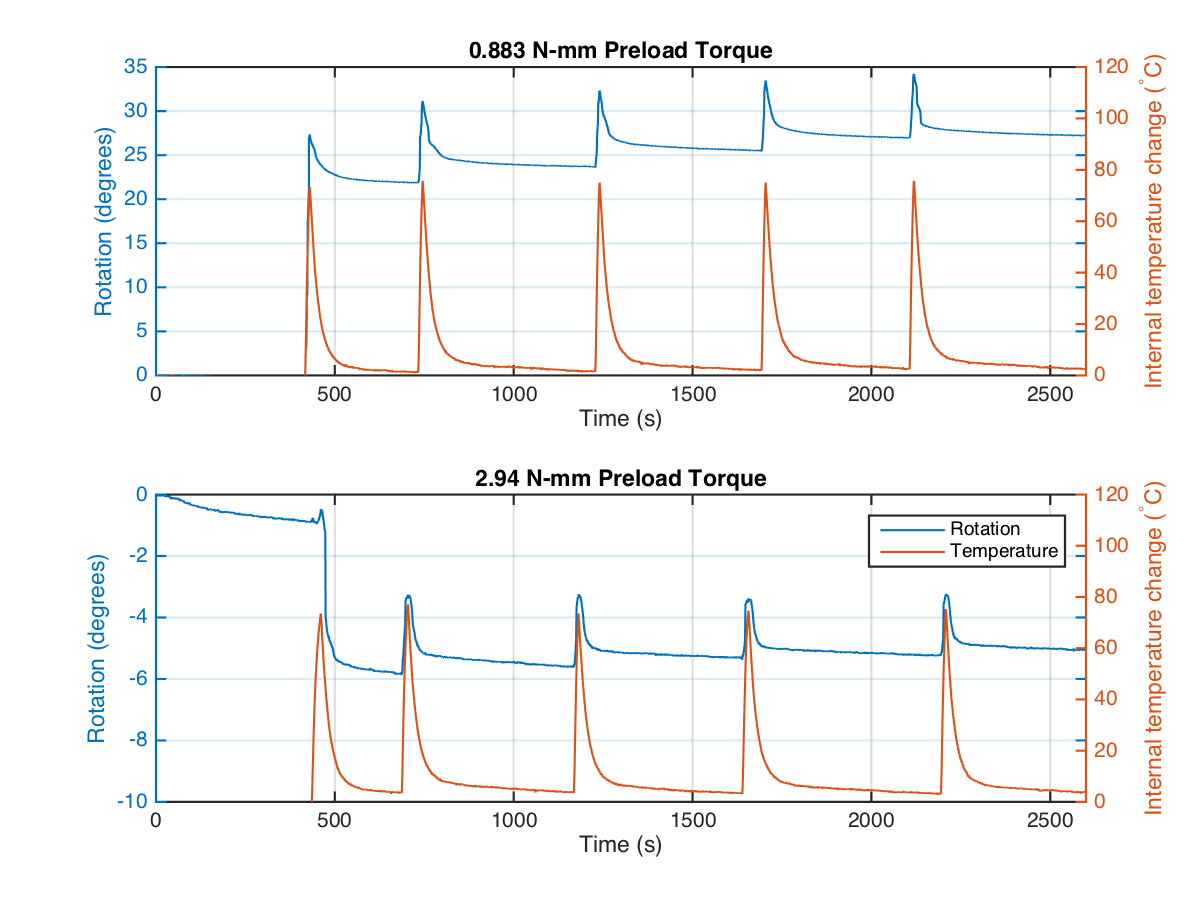
\includegraphics[width=9cm,clip = true, trim = {1cm, 0 ,0 ,0 }]{../Images/TIMEPLOT_030100M.png}
        \caption{Angular displacement and temperature as a function of time for three cycles of actuation for two different torsional preloads. }
        \label{fig:time_hist}
\end{figure}
\begin{figure}
    \centering
        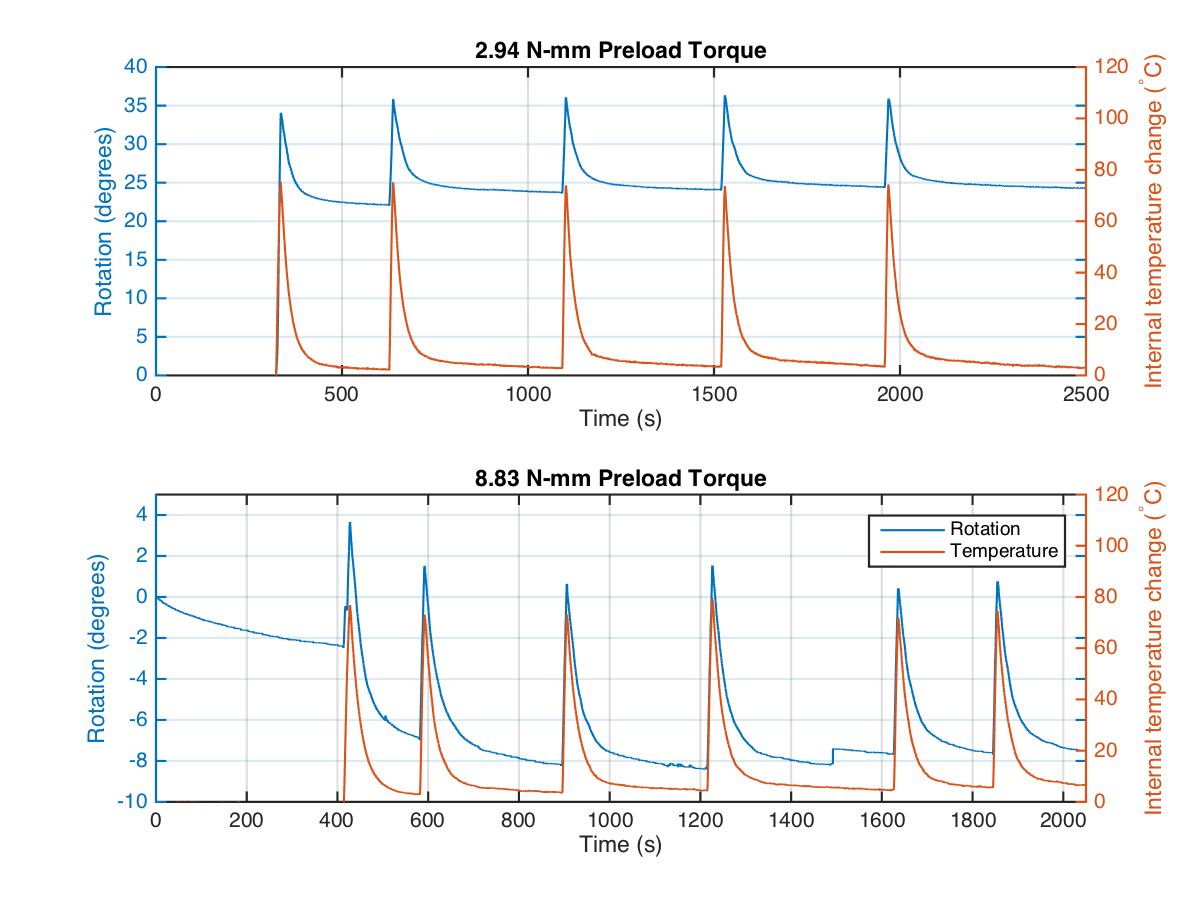
\includegraphics[width=9cm,clip = true, trim = {1cm, 0 ,0 ,0 }]{../Images/TIMEPLOT_100300P.png}
        \caption{Angular displacement and temperature as a function of time for three cycles of actuation for two different torsional preloads. }
        \label{fig:time_hist}
\end{figure}

\begin{figure}
    \centering
        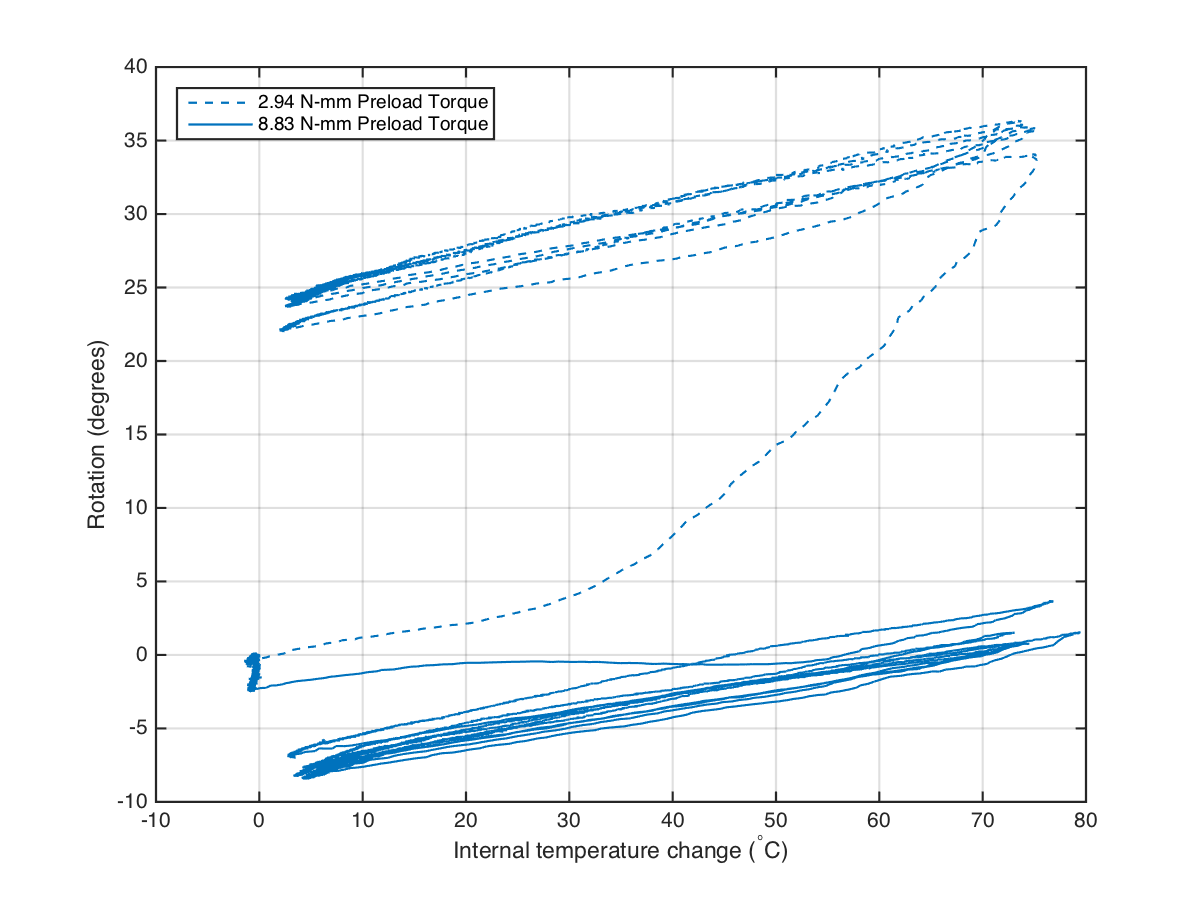
\includegraphics[width=9cm,clip = true, trim = {1cm, 0 ,0 ,0 }]{../Images/ROT_V_TEMP_100300P.png}
        \caption{Angular displacement versus temperature for three cycles of actuation for two different torsional preloads. }
        \label{fig:coiled}
\end{figure}


\section{Discussion}

There are several observations from these experimental results that have important consequences for the design of STPA torsional actuators.  The most apparent is the ``first cycle effect'', where the STPAs behave differently during the first cycle as compared all subsequent cycles.  In all data, the actuation of STPAs show irreversibly during the first cycle,  whereas in later cycles the STPAs show significantly more recovery.  The parallel configuration shows full or nearly full recovery after the first cycle whereas the monofilament STPA shows only partial recovery on subsequent cycles at both torque levels.  %could we cite others that have observed this either for other polymers or for other actuators?
Others have observed this first cycle effect in shape-memory polymers (e.g. \cite{Lendlein_Biodegradable}), but it has not been reported for STPAs \cite{Aziz_Controlled}.  In shape-memory polymers this effect is associated with reorientation of the polymer chains and inelastic behavior \cite{Lendlein_Biodegradable}.
The reason for this first cycle effect in TPAs is not completely clear at this point.  We checked to see if precursor (untwisted) fibers fully recover after thermal loading under no stress, and they do within 1 or 2\%, which suggest that thermal loading is generally recoverable in these materials, so the lack of recovery in the first cycle is associated with the twisted configuration and/or the preload.  We also checked to see if plastic deformation was present for the given preloads, as that could be a cause of irreversibly, but plastic deformation was minimal, and even with 8.83 N-mm torque applied the STPA fully recovered from the torsional load within 1 or 2\%, suggesting that plastic deformation due to the torsional load is not fully responsible for the irreversibly.  From a practical standpoint, the first cycle effect requires that STPAs be cyclically stabilized before use if reversibility is desired.  If reorientation of polymer chains is part of the cause of the first cycle, then it would be important to do this cyclic stabilization at the highest torque expected.  

The larger percent recovery in the parallel configuration as compared to the monofilament STPA might be preferable in applications.  %, particularly when larger torsional loads are required.  In addition, 
Moreover, the parallel configuration shows more rotation and higher torques than the monofilament STPA.  The higher torques are expected as multiple STPAs can lift more load than a single STPA.  However, the higher rotation is not necessarily obvious, since the untwist in the STPA is a function of the initial twist during fabrication, material, and radius of the STPA \cite{Aziz_Controlled}, which are all the same for the monofilament STPA and the parallel configuration. 
We think that the additional displacement in the parallel configuration may be due to the helical wrapping of that configuration.  First, the helical wrapping slightly increases the length of the sample in the parallel configuration, which will increase the rotation during actuation.  Next, STPAs want to untwist about their own axis, and for the case of the parallel configuration, this axis is itself twisted, and therefore additional untwist occurs.   

Note that while we refer to untwist as the actuation phenomenon, with the larger applied torque, the STPAs actually twists during actuation.  With both configurations, under the larger torsional preload, before the application of any thermal load, the STPA twists due to the application of the preload.  Then the heat does cause untwist, as evidence by the initial increase in rotation angle with the application of heat, but that untwist is relative to the twist in the STPA after the load is applied.  
For the monofilament STPA, this untwist during the first heating is relatively minor, whereas for the parallel configuration there is more untwist during the first cycle.  Part of what we think may be occurring is that in addition to the untwist, the polymer's elastic modulus changes with temperature \cite{Shafer_first}.  So the material is more complaint with heat,  and thus the load can twist it more.   These competing phenomenon make it such that the STPA can either untwist or twist further due to heating depending on the applied torque.  
This highlights the need to have a model to predict the behavior of STPAs that accounts for this change in modulus as well as the untwisting during heating.  

After the first cycle, even with the largest torques, the monofilament STPA or the parallel configuration untwist about the same during each cycle.  
With the parallel configuration approximately 10-15$^\circ$ of rotation is seen in subsequent cycles,  and for the monofilament approximately 2-9$^\circ$ of rotation is seen in subsequent cycles.    In addition, Fig. \ref{fig:????} shows that the slope of the rotation vs. temperature curve is nearly the same for both preloads in the parallel configuration.  This suggest that after the first cycle, the rotation is primarily a function of the twist inserted in the STPA during fabrication and the length of the STPA sample.  In addition Aziz et al. \cite{Aziz_Controlled} showed that the fiber radius significantly effects the actuation stroke.  
The initial twist in both configurations is relatively low (approximately 30$^\circ$).  We expect that higher initial twist in the material will lead to higher actuation stroke, and can be achieved by fabricating the STPA under tensile load.   Furthermore, tension on the STPA during fabrication may effect the thermal expansion of the polymer, and thus the rotation during actuation, if it is subject to the Gough-Joule effect.  



Stick-slip is apparent, to various degrees, in all results. This is seen as a jump or jag in the rotation vs. time curve while temperature is changing smoothly.  We think this is an artifact of the experimental set-up and not a property of the material.  In particular, the weight which served to apply the torque was guided and we think that guide got stuck.  In future experiments, we will redesign this guide in order to minimize friction.  


%When comparing the monofilament STPA to the parallel configuration, it can be seen that the parallel configuration  is more stable and can recover fully with larger torques, however, the monofilament STPA has less hysteresis in the rotation vs. temperature change.  %, and has higher rotation under the same torque.  The parallel configuration shows complete reversibility under 8.83 N-mm preload, whereas the monofilament STPA shows more variable amounts of reversibility under that same load.  Under the 2.94 N-mm preload, both the monofilament STPA and the parallel configuration show some drift in the reversiblity, suggesting some sort of relaxation of the material under this smaller torsion.  % more variability in the degree to which it the actuation is reversible.  


%The major drawback of the parallel configuration is the hysteresis in the rotation vs. temperature curve.  This hysteresis is likely explained by the friction between the fibers and the heating wire in the parallel configuration, which is not present in the monofilament, which is why the monofilament shows little hysteresis.  
%It is interesting to note that shape of the rotation vs. temperature curves are quite similar for the two different preloads for each configuration.  That suggest that the energy losses are similar regardless of the preload. 


%Aziz et al. \cite{Aziz_Controlled} were able to get torional actuation on the order of 100$^\circ$, 

Finally, while we used forced air to heat the STPAs, the heating wire embedded in the parallel configuration may serve as a better heating source in applications.   However, with the heating wire thermal conductivity might limit the actuation of STPAs.  Future work will investigate this and the general effectiveness of wire as a heat source for STPA.  %This should be throughly investigated.  
 In addition, forced air or water cooling could significantly increase the time for actuation, but would require significant input energy and additional design challenges.


%Things to mention:
%	Very little tension applied when fabricating actuation - reduced polymer chain angle- reduced perfomance
%	Force air or water cooling would significantly increase actuation cycle times. 
% 	Precycling is needed for low actuators with low preloads
%	It is interesting that the actuation angle on subsequent cycles of low preloads come back to the same max angle as the initial deformation. 
%	
%	
%	
%	Plastic deformation appears to be minimal in the 300 g preload test
%	Some irreversible deformation on straight fibers when heated and then cooled, but this is also minimal. 
%
%	parallel configuration seems to create higher actuation angles and better recovery. 

\section{Conclusions}

In this work we showed that thermally activated torsional actuation is possible with twisted nylon monofilament in two different configurations: a parallel configuration that uses three STPA monofilaments, each twisted about their own axis and twisted together, and a single monofilament of STPA that is twisted about its own central axis.  During the torsional actuation there is not full recovery during the first cycle, but upon subsequent cycles, the recovery is full or nearly full.  This suggests the importance of cyclically stabilizing the TPA prior to use.  The parallel configuration shows higher torsional stroke and better recovery, suggesting that it may be preferable for applications.  Furthermore, the parallel configuration embeds a heating wire, which can be used to apply the thermal load.  While, the majority of testing in this work used forced air to heat the STPAs, we were able to use the heating wire to show that it is possible to use this thermal source in applications.  



\bibliography{../../../LITERATURE/ALL_REFS}

\bibliographystyle{asmems4}





\end{document}

